\chapter{Evaluation}\label{ch:evaluation}

In our tool, usability and user experience are very important. Therefore, we did two user studies. The first was to test the functionality of the GuideaMaps (as map creator and as end-user), while the second tested the use case about Plateforme DD.\\

This chapter is divided in two sections. The first describes the user study of GuideaMaps together with its results. In the second section, the same is done for the user study of Plateforme DD.





\section{GuideaMaps}

\subsection{Tasks \& Questions}

\subsection{Results}





\section{Plateforme DD}
The evaluation of the use case about Plateforme DD is different in comparison to the one about GuideaMaps. A first difference is that our audience is different: for GuideaMaps we chose for participants with a background in Computer Science to take the role as map creator. The participants taking the role of end-user were also more than 20 years old. Now, for Plateforme DD, our audience is between ten and fifteen years old. This is because the content on the website\footnote{\url{https://sciences.brussels/dd/}} was created by children of similar ages \textcolor{red}{(TODO: check this)}. However, the participants of the user study never worked with the website before.

\subsection{Setup}
The children were divided in two groups: one group solved the questionnaire using the website, while the other group solved the same questionnaire using the application. There was one tablet per two children on which the website or the application was running (depending on the group they were in). It was important they did not work with both systems because then there was the possibility a learning effect of having used one system before the other could influence the results. 

\subsection{Tasks \& Questions}
The user study consisted of different tasks and questions the children had to solve. Before they started with the actual tasks and questions, we gave them five minutes to explore the website or the application so that they could get used to it a bit. We mentioned that it was important to understand the structure as much as possible because some questions would follow after this introduction period.\\

After five to ten minutes, we distributed the papers with the tasks and the questions. With other words, all children (of both groups) received part 1 of the questionnaire (see \autoref{appendix:pdd-questionnaire}). The first six questions of part 1 were about the understanding of the structure of the content. Then, four more questions were added to test the searching and finding of information in both systems. The participants using the application also had to answer four more questions about ``insight'' in the way the information is structured and linked. Participants using the website did not have to answer these questions because these are specific for the application.\\

After twenty minutes, all questionnaires of part 1 were collected, even if the participant did not finish all questions yet. Together with the pages, the tablets were collected as well because there are no questions left where the participants really needed the application or the website anymore. After collecting everything, part two of the questionnaire was distributed to all participants. In this part, the questions were not about the content or the structure of the information, but about usability and user experience. Hence, we wanted to know the opinion of the participants about the system they used so that we could compare which of the two systems they liked the most. The questions about usability and user experience can be found in \autoref{appendix:pdd-questionnaire} and \autoref{appendix:ueq-questionnaire}, respectively. The usability questions are based on the SUS questionnaire\footnote{\url{https://www.usability.gov/how-to-and-tools/methods/system-usability-scale.html}}. We adapted the questions a bit because not all questions were useful for our purpose.



\subsection{Results}
In general, we predict that participants using the application are better in answering most of the questions of part 1 correctly than the participants using the website. Certainly because they only have 20 minutes to answer all questions. We expect that not all participants using the website will be able to answer all questions in this amount of time. Even though we know it is possible that some participants using the application will not be able to finish the questionnaire either, we predict participants using the application will be able to answer more of the questions than participants using the website.

\subsubsection{Structure Comprehension}

\begin{figure}[H]
	\centering
	\frame{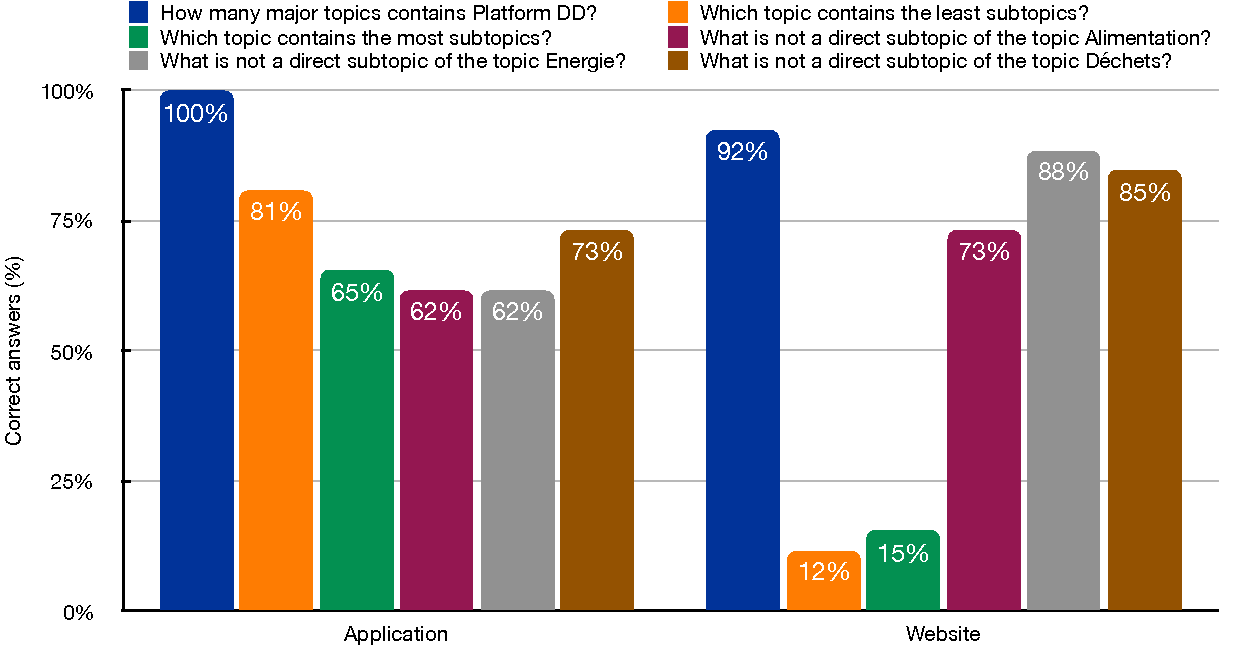
\includegraphics[width=\linewidth]{evaluation/part1-first6.pdf}}
	\caption{Results of the first 6 questions of part 1.}
	\label{fig:evaluation-first6}
\end{figure}

\autoref{fig:evaluation-first6} shows the results of the first six questions of the questionnaire. We can see that almost every participant correctly found that the content is divided over three major topics. But more important is that participants using the application were significantly better in finding which topic contains the most and which the least number of subtopics. We expected this because in the application, the tree structure is more clear. As a consequence, these users have a better overview than the participants using the website. To the questions about which is not a direct subtopic of a certain topic, the participants using the website gave a correct answer more frequently. This is probably because these users cannot see indirect subtopics of the topics in the questions. Participants using the application possibly made some indirect subtopics visible by clicking on the plus-button and were then a bit disturbed.

\subsubsection{Search \& Find}
After the first six questions, in which they discovered the structure of the content, we asked them to search and find information in the tool they were using. The results can be found in \autoref{fig:evaluation-search-find}. In general, we see that participants using the application are better in retrieving the information from the tool than the ones using the website.

\begin{figure}[H]
	\centering
	\frame{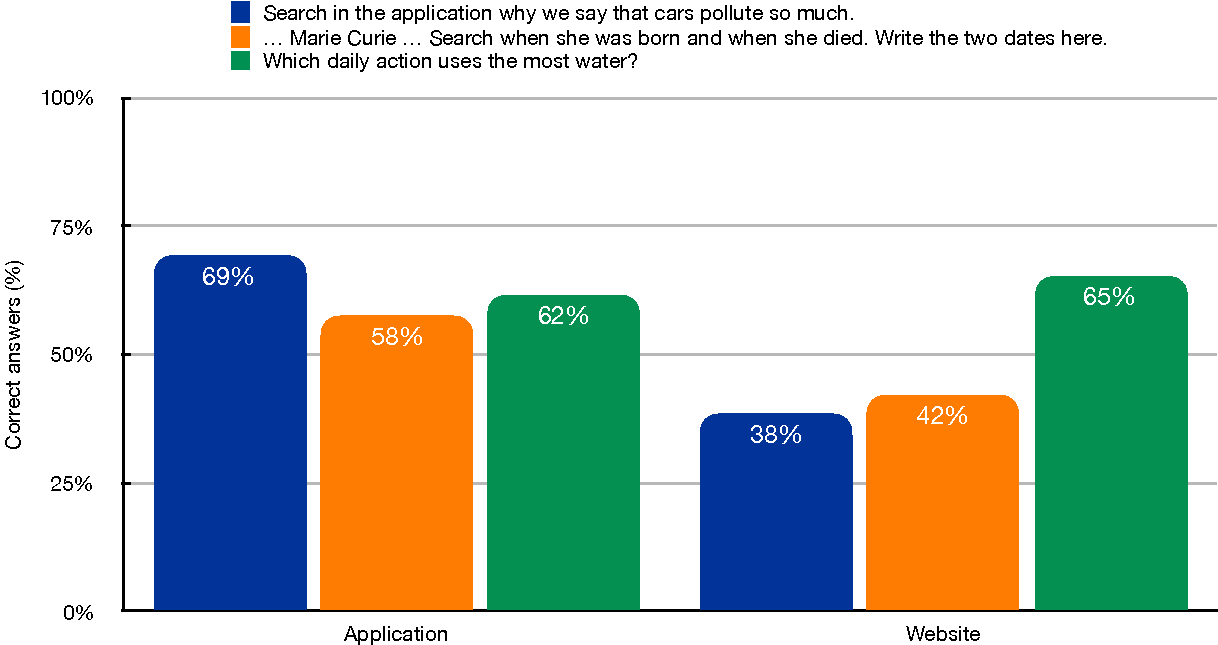
\includegraphics[width=\linewidth]{evaluation/part1-search-find.pdf}}
	\caption{Results of search \& find questions.}
	\label{fig:evaluation-search-find}
\end{figure}

We also asked them to write the titles as possible of topics which are still ``under construction''. This was not very successful because more than half of the participants could not find such a topic. The average number of topics found per participant is 0.42 in the case of the application and 0.81 in case of the website. This is probably because going through the topics on the website is quite fast, i.e. you just click on other topics until you find one that is under construction, while in the application you have to open and close the nodes one by one which takes more time.

\subsubsection{Insight}
The participants using the application had to answer four additional multiple choice questions to test their insight about the tool.

\begin{figure}[H]
	\centering
	\frame{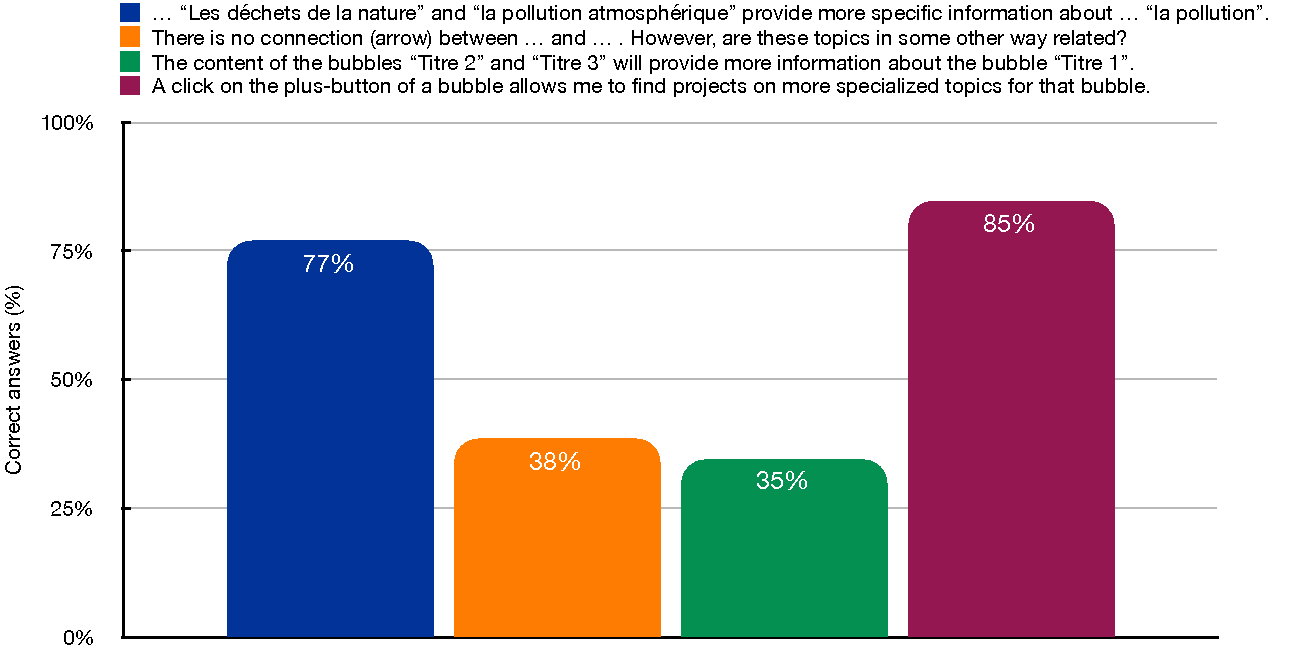
\includegraphics[width=\linewidth]{evaluation/part1-insight.pdf}}
	\caption{Results of insight questions.}
	\label{fig:evaluation-insight}
\end{figure}




%\begin{figure}[H]
%	\centering
%	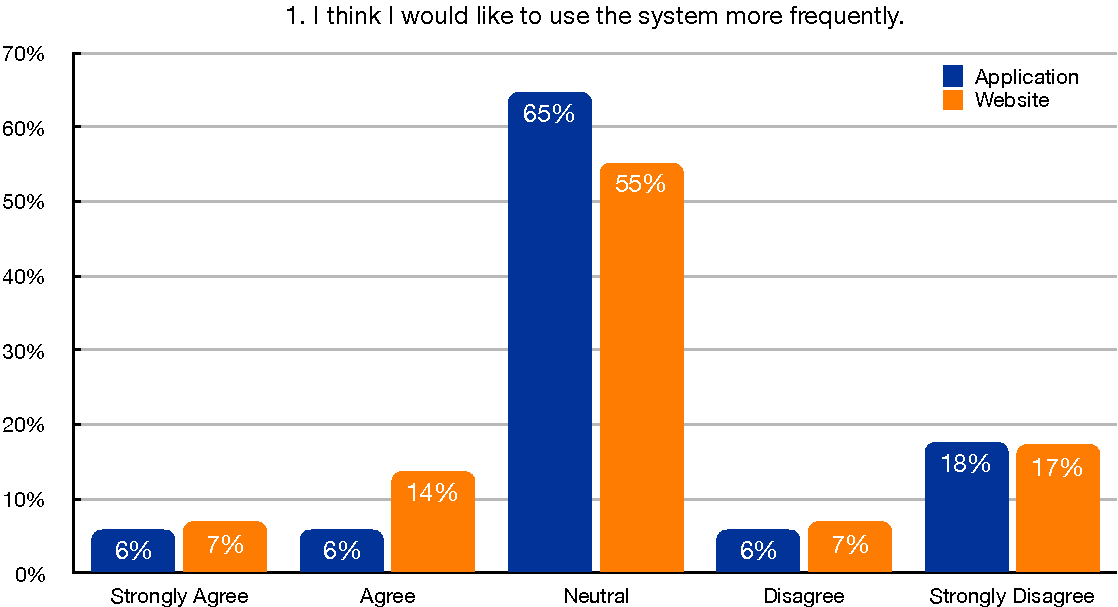
\includegraphics[width=.49\textwidth]{evaluation/usability-q1.pdf}
%	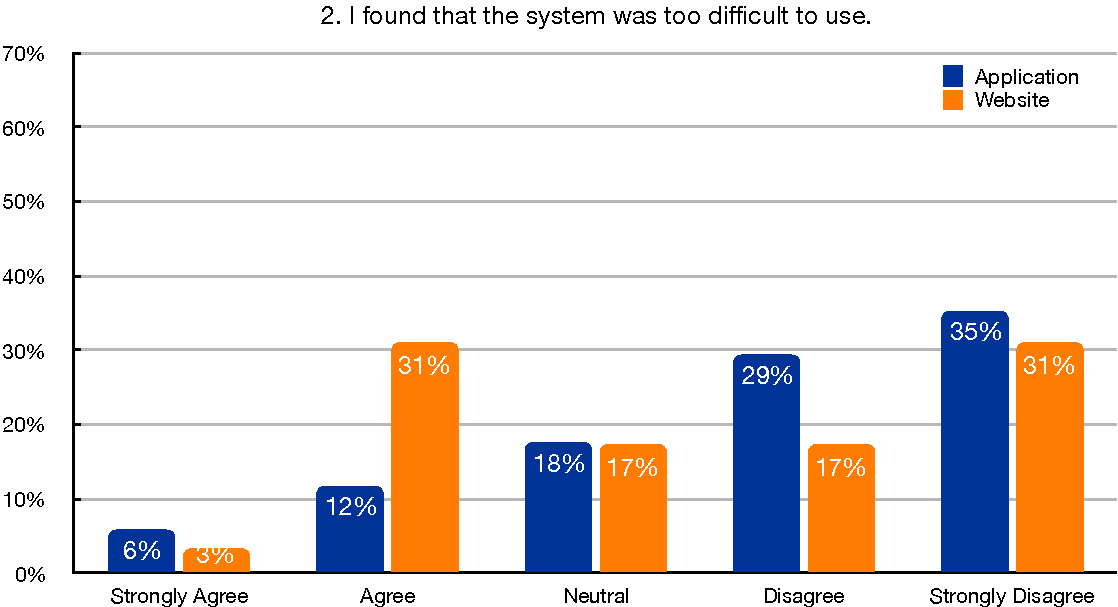
\includegraphics[width=.49\textwidth]{evaluation/usability-q2.pdf}
%	
%	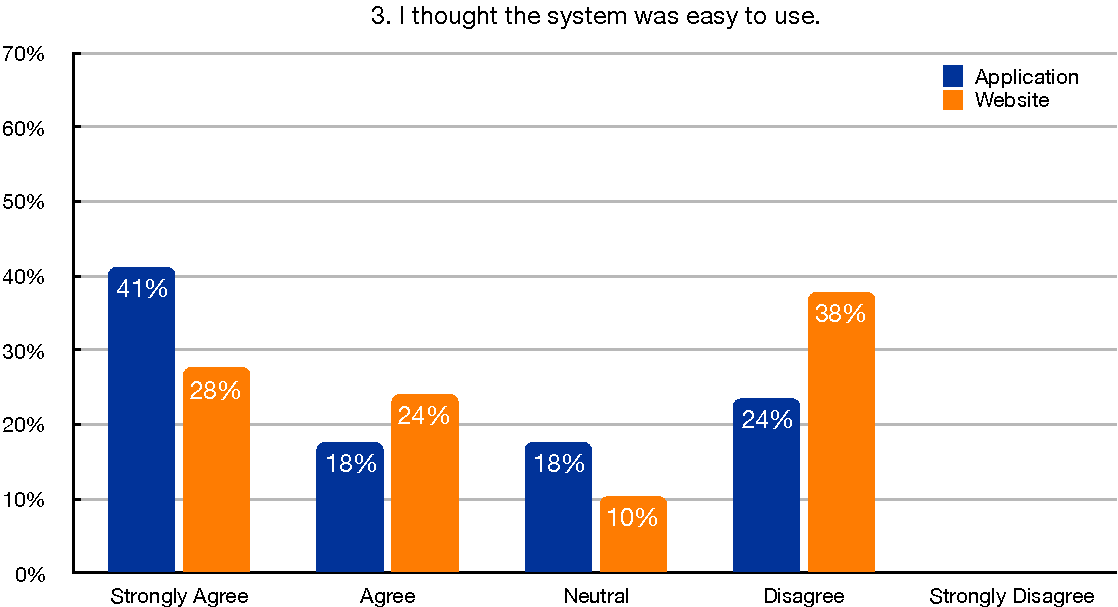
\includegraphics[width=.49\textwidth]{evaluation/usability-q3.pdf}
%	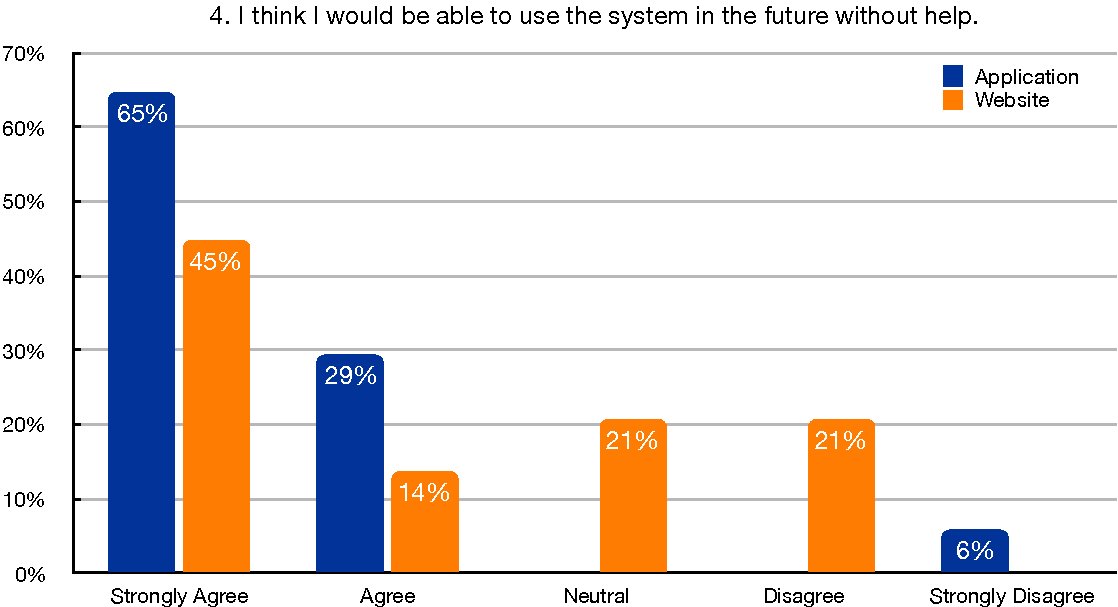
\includegraphics[width=.49\textwidth]{evaluation/usability-q4.pdf}
%	
%	\caption{test}
%\end{figure}

\subsubsection{Usability}
For the second part of the questionnaire, we expect the website is less usable than the visualization. Further, because we had more difficulties to search and find information on the website than in the application, we expect the user experience of the application will be better in comparison to the website.

\begin{figure}[h]
	\centering
	\begin{subfigure}{.49\textwidth}
  		\centering
  		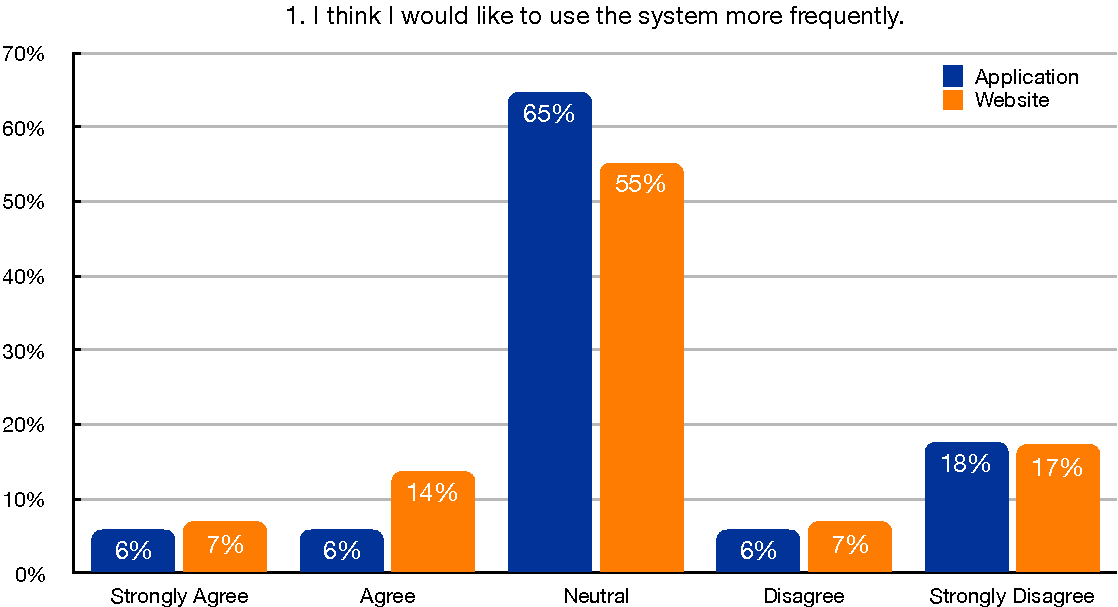
\includegraphics[width=\linewidth]{evaluation/usability-q1.pdf}
  		\caption{Results for question 1.}
  		%\label{fig:plusicon}
	\end{subfigure}%
	\begin{subfigure}{.49\textwidth}
  		\centering
  		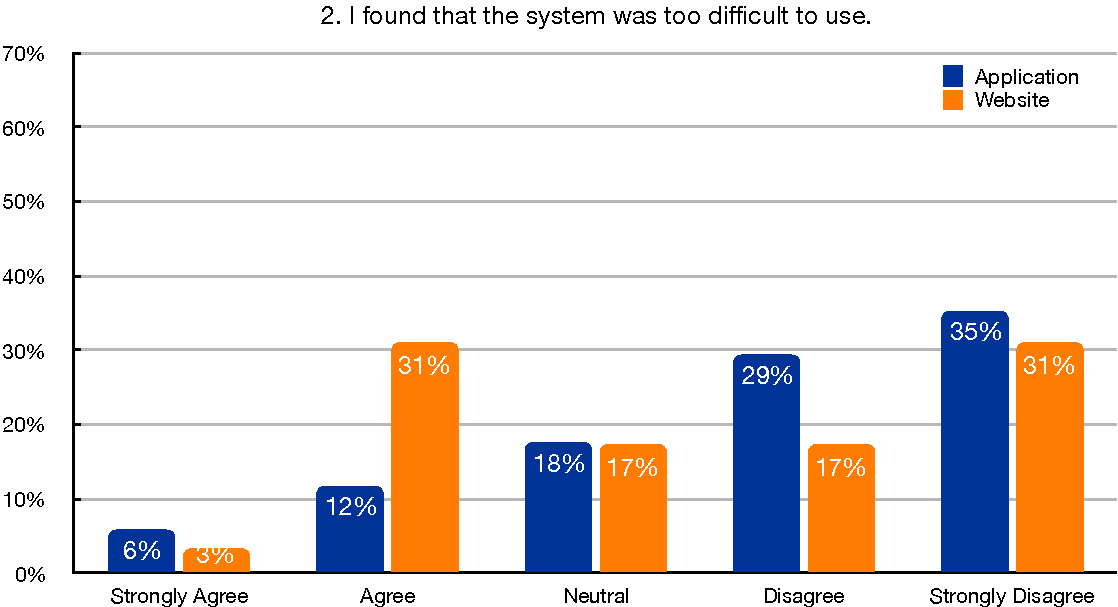
\includegraphics[width=\linewidth]{evaluation/usability-q2.pdf}
  		\caption{Results for question 2.}
  		%\label{fig:editicon}
	\end{subfigure}\par\bigskip
	
	\begin{subfigure}{.49\textwidth}
  		\centering
  		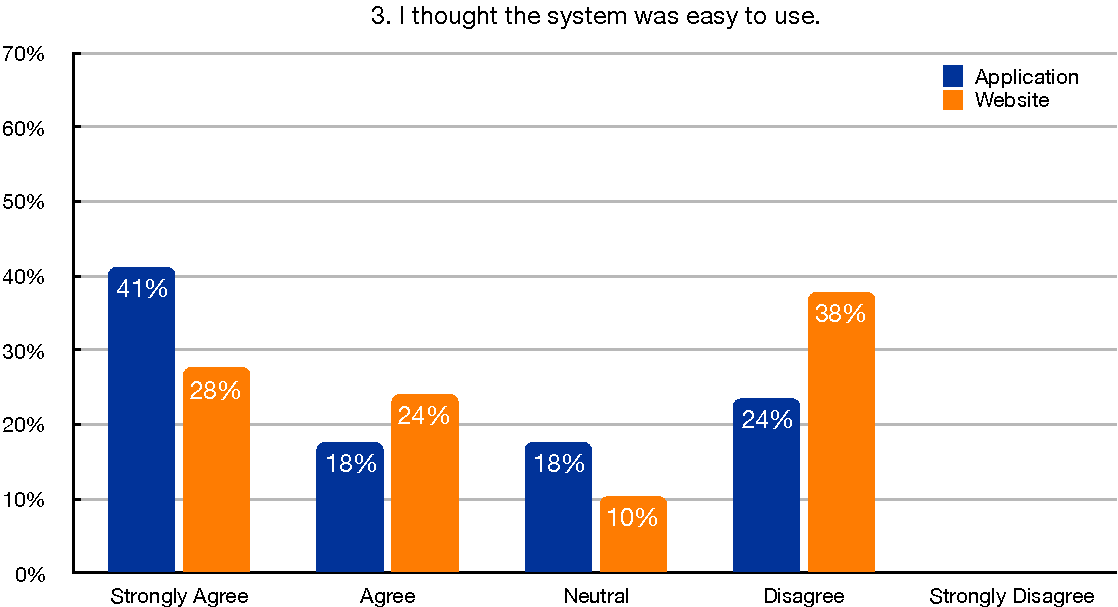
\includegraphics[width=\linewidth]{evaluation/usability-q3.pdf}
  		\caption{Results for question 3.}
  		%\label{fig:plusicon}
	\end{subfigure}%
	\begin{subfigure}{.49\textwidth}
  		\centering
  		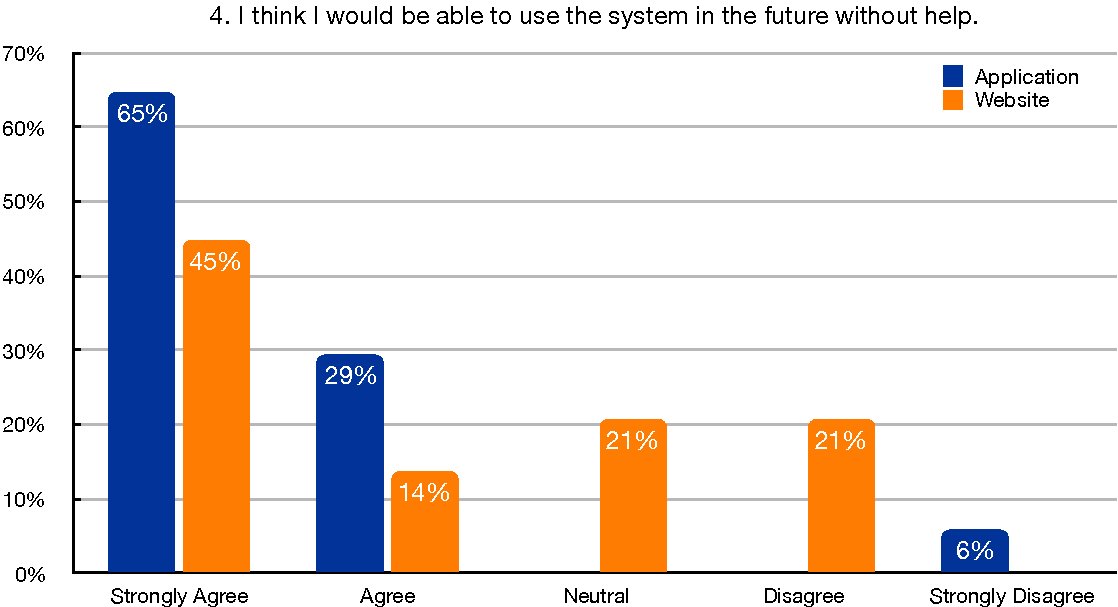
\includegraphics[width=\linewidth]{evaluation/usability-q4.pdf}
  		\caption{Results for question 4.}
  		%\label{fig:editicon}
	\end{subfigure}\par\bigskip
	
	\begin{subfigure}{.49\textwidth}
  		\centering
  		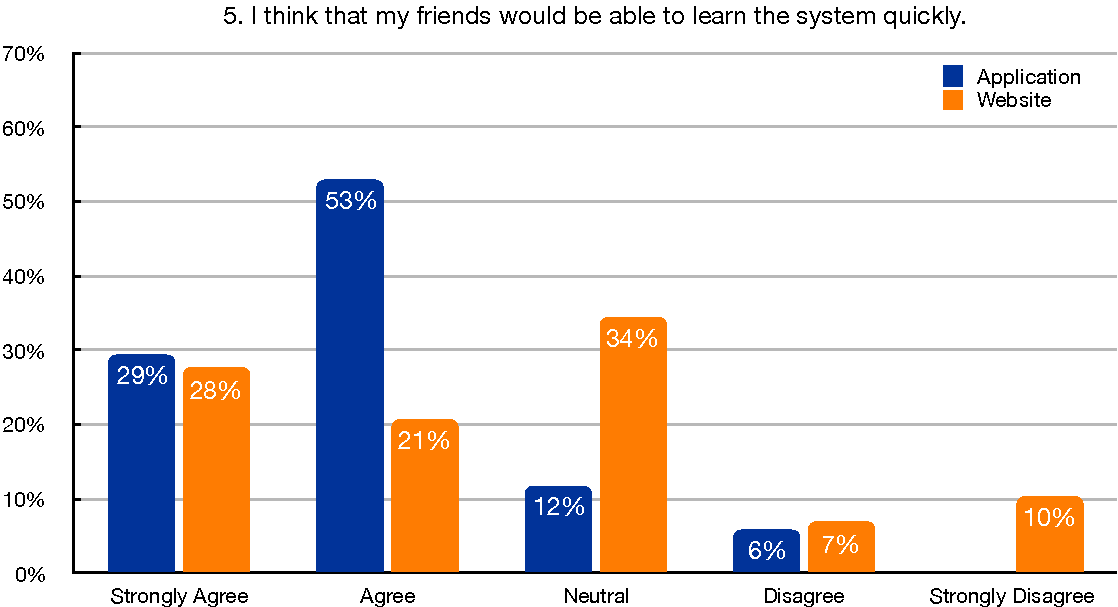
\includegraphics[width=\linewidth]{evaluation/usability-q5.pdf}
  		\caption{Results for question 5.}
  		%\label{fig:plusicon}
	\end{subfigure}%
	\begin{subfigure}{.49\textwidth}
  		\centering
  		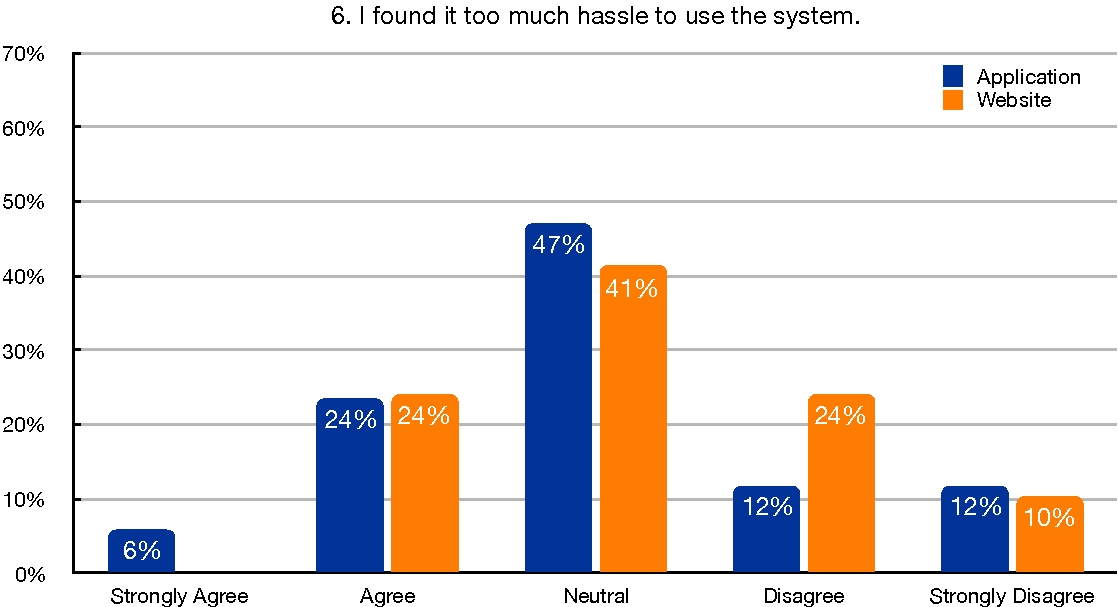
\includegraphics[width=\linewidth]{evaluation/usability-q6.pdf}
  		\caption{Results for question 6.}
  		%\label{fig:editicon}
	\end{subfigure}\par\bigskip
	
	\begin{subfigure}{.49\textwidth}
  		\centering
  		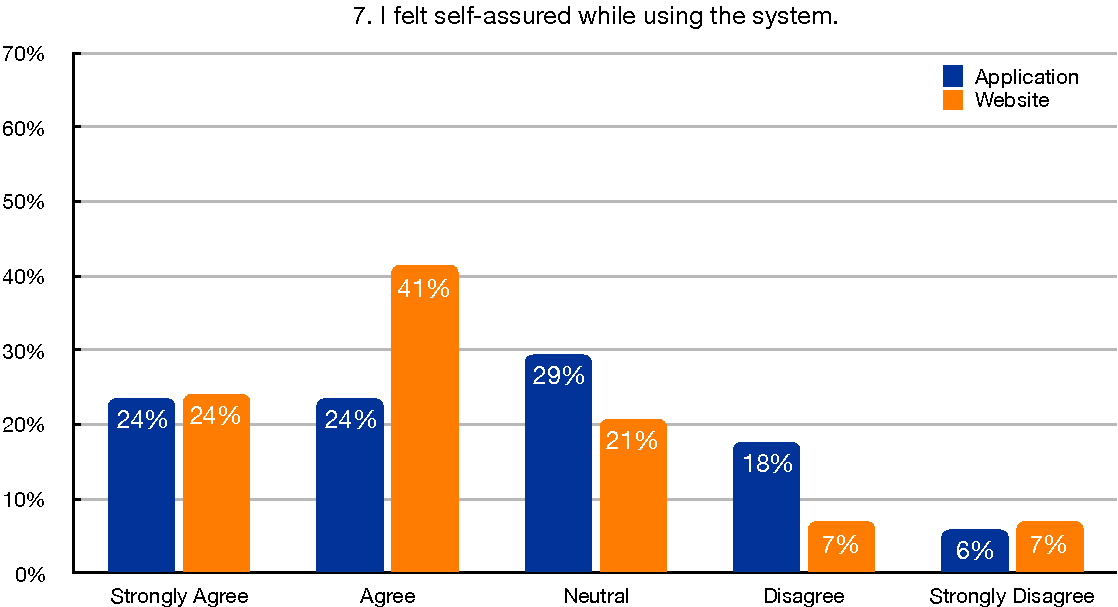
\includegraphics[width=\linewidth]{evaluation/usability-q7.pdf}
  		\caption{Results for question 7.}
  		%\label{fig:plusicon}
	\end{subfigure}%
	\begin{subfigure}{.49\textwidth}
  		\centering
  		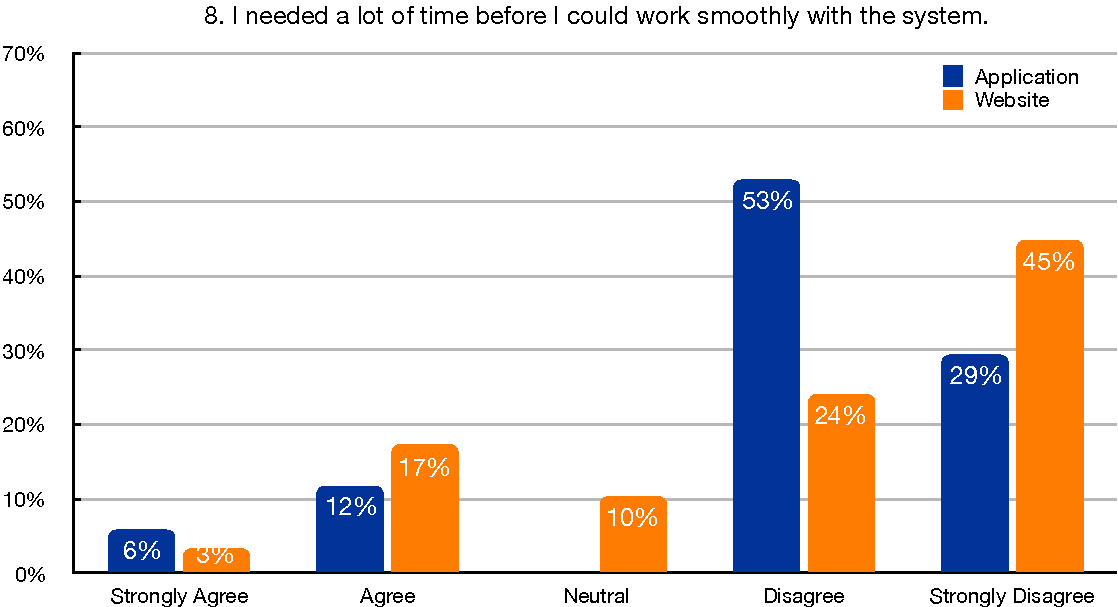
\includegraphics[width=\linewidth]{evaluation/usability-q8.pdf}
  		\caption{Results for question 8.}
  		%\label{fig:editicon}
	\end{subfigure}
	\caption{Results of all eight usability questions.}
	%\label{fig:icons}
\end{figure}

\subsubsection{User Experience}
To test the user experience, we used a questionnaire\footnote{\url{https://www.ueq-online.org/}} composed in such a way that inconsistencies can be easily detected. Together with the questionnaire, you can download an excel-file in which you have to insert all given answers. In the file, the answers are immediately analyzed and graphs are created for you.






